\scanpage{8}
% archive sheet number: 7
\[
\mathrm{R}\handwritten{(}gf_{\deleted{\unsure{!|*}}}\handwritten{)}_{\handwritten{!}}(F_X)\handwritten{\longrightarrow}\mathrm{R}g_{\handwritten{!}}(F_Y)(d'-d)\handwritten{[}2(d'-d)\handwritten{]}\deleted{\unsure{,|.}},
\tag*{(4.2.3)}
\]
déduit de (4.2) en appliquant $\mathrm{R}g_{\handwritten{!}}$. De même, appliquant $\mathrm{R}g_*$, on trouve
\[
\mathrm{R}g_*\mathrm{R}f_{\handwritten{!}}(F_X)\overset{\mathrm{dfn}}{=}\mathrm{R}(gf)_{\deleted{\unsure{!|f}}c(f)}(F_X)\handwritten{\longrightarrow}\mathrm{R}g_{\handwritten{*}}(F_Y)(d'-d)\handwritten{[}2(d'-d)\handwritten{\unsure{]} }
\tag*{(4.2.4)}
\]
(où l\unsure{\deleted{e}a|\deleted{a}e} \deleted{premier}\inserted{source} est ``l'image directe à supports propres sur $Y^{\deleted{\unsure{*|k|''}}}$'' )\deleted{\unsure{, qui,}}

\deleted{Prenant en particulier} Pour définir cette dernière flèche, \deleted{il était}\inserted{quitte à faire rentrer le $(d'-d)$ dans la parenthèse, il} suffisait de disposer d'un morphisme de \deleted{sites} topos $Y_{\text{ét}}\handwritten{\longrightarrow}Z$, et prenant alors pour $Z$ le topos final, on trouve l'exemple important d'homomorphisme de Gysin:
\[
\mathrm{R}\handwritten{\Gamma}_X(\mathrm{R}f_{\handwritten{!}}(F_X))\overset{\mathrm{dfn}}{=}\mathrm{R}\handwritten{\Gamma}_{X,\deleted{\unsure{!|f}}c(f)}(F_X)\handwritten{\longrightarrow}\mathrm{R}\handwritten{\Gamma}_Y(F_Y(d'-d))\handwritten{[}2(d'\unsure{\mathord{\perp}|-}d)\handwritten{\unsure{]} }
\tag*{(4.2.5)}
\]
Dans le cas où $f$ est \uline{propre}, (4.2) devient
\[
\mathrm{R}f_{\handwritten{*}}(F_X)\handwritten{\longrightarrow}\mathbb{F}_Y(d'-d)\handwritten{[}2(d'-d)\handwritten{]},
\tag*{(4.2.\unsure{6|5})}
\]
et (4.2.4) et (4.2.5) s'écrivent respectivement
\[
\mathrm{R}(gf)_*(F_X)\handwritten{\longrightarrow}\mathrm{R}g_{\handwritten{*}}(F_Y)(d'-d)\handwritten{[}2(d'-d)\handwritten{]},
\tag*{(4.2.7)}
\]
\[
\mathrm{R}\handwritten{\Gamma}_X(F_X)\handwritten{\unsure{\text{---}|\longrightarrow}}\mathrm{R}\Gamma_Y(F_Y(d'-d))\handwritten{[}2(d'-d)\handwritten{]}.
\tag*{(4.2.8)}
\]

\deleted{Dans (4.2.5) ou (4.2.8), il y aurait lieu de remplacer $F_X$ par un $F_X(i)$} On a également à définir des homomorphismes de Gysin pour des coéfficients sur $Y$ plus généraux que ceux de la forme $F_Y$ et ceux qu'on en déduit par twist et shift. De façon générale, soit $G$\unsure{.|:|;} un complexe de $A$-Modules (NB je ne précise pas ici\inserted{ni ailleurs} les hypothèses de degré) sur $Y$, et appliquons à (4.2) le foncteur $\overset{\mathrm{L}}{\otimes}G$, on trouve un homomorphisme canonique, qui est d'ailleurs le même que si on partait de \deleted{F} $F'=A_S$ sur $S$, et qu'on tensorise l'homomorphisme de Gysin correspendant par $F_Y\otimes G$. Donc, autant oublier $F$ et dire que pour tout $G$ sur $Y$, on a un homomorphisme canonique (dit\inserted{\handwritten{encore}} \uline{de Gysin})
\margin{\begin{tikzpicture}[x=1cm,y=1cm,baseline=(note.north)]
\node[anchor=north west,align=left,inner sep=0] (note) at (0,0) {\handwritten{Question: a-t-on\\besoin d'un $A$ sur $S$,\\\unsure{ou|ne} suffit d'avoir\\un Anneau $A_Y$\\sur $Y$, de torsion,\\premier à $\unsure{Y|\zeta}$ ?}};
\draw[line width=.45pt] (-.08,.18) .. controls (1.4,.27) and (3.35,.58) .. (4.25,.22) .. controls (4.85,.02) and (5.17,-.38) .. (5.17,-.81) .. controls (5.14,-1.47) and (4.85,-2.35) .. (5.13,-2.58) .. controls (5.37,-2.76) and (5.86,-2.65) .. (6.10,-2.96) .. controls (6.34,-3.19) and (6.25,-3.52) .. (6.27,-3.83);
\end{tikzpicture}}
\figure{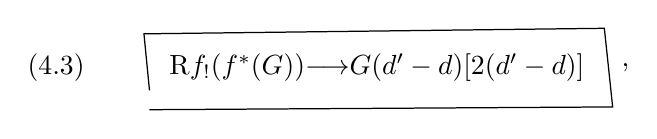
\begin{tikzpicture}[x=1cm,y=1cm,baseline=(formula.base)]
\node[anchor=west,inner sep=0] at (-1.8,0) {$(4.3)$};
\node[anchor=west,inner sep=0] (formula) at (0,0) {$\mathrm{R}f_{\handwritten{!}}(f^{\handwritten{*}}(G))\handwritten{\longrightarrow}G(d'-d)\handwritten{[}2(d'-d)\handwritten{]}$};
\draw[line width=.45pt] ([xshift=-7pt,yshift=-3pt]formula.south west) -- ([xshift=-9pt,yshift=7pt]formula.north west) -- ([xshift=7pt,yshift=9pt]formula.north east) -- ([xshift=10pt,yshift=-9pt]formula.south east) -- ([xshift=-7pt,yshift=-10pt]formula.south west);
\node[anchor=west,inner sep=0] at ([xshift=13pt]formula.east) {,};
\end{tikzpicture}}
ou, au choix
